%% Patent Application: Closed-Loop Isothermal-Resonant Control Algorithms
%% for Protein Folding Modulation
%% Inventor: Jonathan Washburn
%% Contact: washburn.jonathan@gmail.com
%% Filing Date: January 2026

\documentclass[12pt,letterpaper]{article}

\usepackage[margin=1in]{geometry}
\usepackage{amsmath,amssymb,amsfonts}
\usepackage{graphicx}
\usepackage{tikz}
\usetikzlibrary{shapes,arrows,positioning,calc,patterns}
\usepackage{booktabs}
\usepackage{array}
\usepackage{enumitem}
\usepackage{fancyhdr}
\usepackage{xcolor}
\usepackage{hyperref}
\usepackage{setspace}

% Patent-style formatting
\setlength{\parindent}{0.5in}
\setlength{\parskip}{0.5em}
\onehalfspacing

% Header
\pagestyle{fancy}
\fancyhf{}
\rhead{Patent Application}
\lhead{Washburn}
\rfoot{Page \thepage}

\hypersetup{
    colorlinks=true,
    linkcolor=blue,
    urlcolor=blue,
    citecolor=blue
}

% Custom colors
\definecolor{control}{RGB}{50,100,200}
\definecolor{feedback}{RGB}{200,100,50}
\definecolor{setpoint}{RGB}{50,180,50}
\definecolor{objective}{RGB}{150,50,150}

\begin{document}

%% ============================================================================
%%                              TITLE PAGE
%% ============================================================================

\begin{center}
\vspace*{0.8in}

{\LARGE \textbf{PATENT APPLICATION}}

\vspace{0.4in}

{\Large \textbf{CLOSED-LOOP ISOTHERMAL-RESONANT}}

{\Large \textbf{CONTROL ALGORITHMS FOR}}

{\Large \textbf{PROTEIN FOLDING MODULATION}}

\vspace{0.8in}

\textbf{PROVISIONAL PATENT APPLICATION}

\vspace{0.5in}

\begin{tabular}{ll}
\textbf{Inventor:} & Jonathan Washburn \\
\textbf{Email:} & washburn.jonathan@gmail.com \\
\textbf{Filing Date:} & January 17, 2026 \\
\textbf{Application Type:} & Utility Patent (Provisional) \\
\textbf{Related Applications:} & Patents 001--005 \\
\end{tabular}

\vspace{0.8in}

\textit{Control algorithms for maintaining isothermal conditions while maximizing resonant protein folding modulation, including multi-input multi-output (MIMO) feedback control, multi-objective optimization, adaptive gain scheduling, model predictive control, and real-time constraint satisfaction.}

\vfill

\textbf{CONFIDENTIAL --- PATENT PENDING}

\end{center}

\newpage

%% ============================================================================
%%                         TABLE OF CONTENTS
%% ============================================================================

\tableofcontents
\newpage

%% ============================================================================
%%                              ABSTRACT
%% ============================================================================

\section*{ABSTRACT OF THE DISCLOSURE}
\addcontentsline{toc}{section}{ABSTRACT OF THE DISCLOSURE}

Control algorithms for closed-loop operation of protein folding modulation apparatus, enabling simultaneous isothermal maintenance and resonant modulation maximization. The algorithms comprise: (a) multi-input multi-output (MIMO) feedback control using temperature and folding signal readouts to adjust microwave power, frequency, and cooling power; (b) multi-objective optimization that minimizes temperature deviation $\Delta T$ while maximizing folding modulation $M$, with configurable weighting; (c) adaptive gain scheduling that adjusts control parameters based on operating conditions; (d) model predictive control (MPC) using a thermal-optical model to anticipate system response; (e) constraint satisfaction algorithms ensuring temperature bounds, power limits, and safety interlocks; (f) resonance-tracking algorithms that maintain optimal frequency despite system drift; and (g) isotope-mode switching that automatically reconfigures control parameters for D$_2$O operation. The algorithms enable unambiguous discrimination between resonant and thermal effects by maintaining strict temperature control ($|\Delta T| < 0.1^\circ$C) while achieving significant folding modulation ($M > 30\%$). Implementation may be on embedded controllers, FPGAs, or host computers. Applications include automated protein folding modulation for research, manufacturing, and therapeutic use.

\vspace{1em}
\noindent\textbf{Keywords:} closed-loop control, isothermal, resonant modulation, MIMO, multi-objective optimization, model predictive control, adaptive control, feedback, protein folding

\newpage

%% ============================================================================
%%                      BACKGROUND OF THE INVENTION
%% ============================================================================

\section{BACKGROUND OF THE INVENTION}

\subsection{Field of the Invention}

The present invention relates generally to control systems for scientific instrumentation, and more specifically to closed-loop control algorithms that simultaneously maintain isothermal conditions and maximize resonant modulation of protein folding.

\subsection{Description of Related Art}

\subsubsection{Open-Loop Operation Limitations}

Prior protein folding modulation systems operate in open-loop mode:

\begin{enumerate}[label=(\alph*)]
\item \textbf{Fixed power operation:} Microwave power is set manually without feedback. Temperature drifts during operation.

\item \textbf{Manual frequency selection:} Frequency is set once without real-time optimization. Resonance may drift due to temperature or sample changes.

\item \textbf{Separate temperature control:} Temperature is controlled independently of irradiation, leading to oscillations and overshoot.

\item \textbf{No folding feedback:} The folding signal is measured for data collection but not used to optimize irradiation parameters.
\end{enumerate}

\subsubsection{Limitations of Separate Temperature and Irradiation Control}

When temperature control and irradiation are operated independently:

\begin{enumerate}[label=(\arabic*)]
\item \textbf{Control loop interference:} Microwave heating is treated as a disturbance by the temperature controller, leading to oscillatory behavior.

\item \textbf{Slow response:} Temperature controllers designed for steady-state operation cannot track rapid heating from pulsed irradiation.

\item \textbf{No optimization:} There is no mechanism to trade off temperature stability against modulation effectiveness.

\item \textbf{Thermal-resonant ambiguity:} Without tight temperature control, observed effects may be thermal rather than resonant.
\end{enumerate}

\subsubsection{Prior Art in Laboratory Temperature Control}

Standard laboratory temperature controllers:

\begin{table}[h]
\centering
\begin{tabular}{lll}
\toprule
\textbf{Controller Type} & \textbf{Typical Accuracy} & \textbf{Limitations} \\
\midrule
On-off (bang-bang) & $\pm$2--5$^\circ$C & Large oscillations \\
PID & $\pm$0.1--1$^\circ$C & Slow response to disturbances \\
Cascade PID & $\pm$0.05--0.5$^\circ$C & Complex tuning \\
Water bath & $\pm$0.01--0.1$^\circ$C & Slow thermal mass \\
\bottomrule
\end{tabular}
\caption{Standard laboratory temperature controllers}
\end{table}

None of these controllers are designed for the specific challenge of maintaining isothermal conditions during resonant microwave irradiation.

\subsubsection{The Need for Integrated Control}

What is needed is an integrated control system that:

\begin{enumerate}[label=(\arabic*)]
\item Treats microwave irradiation and temperature control as a \textbf{unified} system;
\item Uses \textbf{multiple feedback signals} (temperature, folding, power);
\item Implements \textbf{multi-objective optimization} balancing thermal stability and modulation;
\item Provides \textbf{model-based prediction} to anticipate heating effects;
\item Ensures \textbf{constraint satisfaction} for safety and isothermal compliance.
\end{enumerate}

\subsection{Objects of the Invention}

It is an object of the present invention to provide control algorithms that:

\begin{enumerate}[label=(\arabic*)]
\item Maintain isothermal conditions ($|\Delta T| < 0.1^\circ$C) during microwave irradiation;
\item Maximize folding modulation subject to isothermal constraints;
\item Adapt to varying operating conditions and sample properties;
\item Predict and compensate for heating effects before they occur;
\item Ensure safe operation through constraint satisfaction;
\item Support both H$_2$O and D$_2$O operation with automatic reconfiguration.
\end{enumerate}

\newpage

%% ============================================================================
%%                      SUMMARY OF THE INVENTION
%% ============================================================================

\section{SUMMARY OF THE INVENTION}

\subsection{General Statement of the Invention}

The present invention provides a family of closed-loop control algorithms for protein folding modulation apparatus, comprising:

\begin{enumerate}[label=(\alph*)]
\item MIMO feedback control architecture;
\item Multi-objective cost function optimization;
\item Adaptive gain scheduling;
\item Model predictive control (MPC);
\item Constraint satisfaction and safety algorithms;
\item Resonance tracking;
\item Isotope-mode automatic reconfiguration.
\end{enumerate}

\subsection{Control System Architecture}

\begin{figure}[h]
\centering
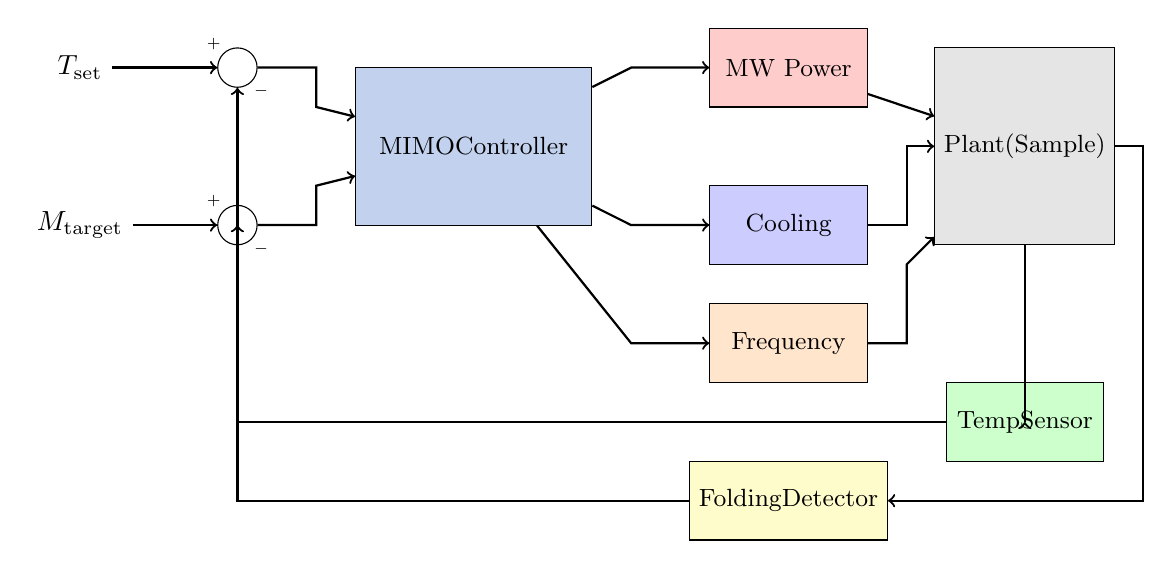
\begin{tikzpicture}[
    block/.style={rectangle, draw, minimum width=2cm, minimum height=1cm, text centered, font=\small},
    sum/.style={circle, draw, minimum size=0.5cm},
    arrow/.style={->, thick}
]
    % Setpoints
    \node (tset) at (-1,3) {$T_{\text{set}}$};
    \node (mset) at (-1,1) {$M_{\text{target}}$};
    
    % Summing junctions
    \node[sum] (sum_t) at (1,3) {};
    \node[sum] (sum_m) at (1,1) {};
    
    % Controller
    \node[block, fill=control!30, minimum width=3cm, minimum height=2cm] (ctrl) at (4,2) {MIMO\\Controller};
    
    % Actuators
    \node[block, fill=red!20] (mw) at (8,3) {MW Power};
    \node[block, fill=blue!20] (cool) at (8,1) {Cooling};
    \node[block, fill=orange!20] (freq) at (8,-0.5) {Frequency};
    
    % Plant
    \node[block, fill=gray!20, minimum width=2cm, minimum height=2.5cm] (plant) at (11,2) {Plant\\(Sample)};
    
    % Sensors
    \node[block, fill=green!20] (tsens) at (11,-1.5) {Temp\\Sensor};
    \node[block, fill=yellow!20] (msens) at (8,-2.5) {Folding\\Detector};
    
    % Arrows - forward path
    \draw[arrow] (tset) -- (sum_t);
    \draw[arrow] (mset) -- (sum_m);
    \draw[arrow] (sum_t) -- (2,3) -- (2,2.5) -- (ctrl);
    \draw[arrow] (sum_m) -- (2,1) -- (2,1.5) -- (ctrl);
    \draw[arrow] (ctrl) -- (6,3) -- (mw);
    \draw[arrow] (ctrl) -- (6,1) -- (cool);
    \draw[arrow] (ctrl) -- (6,-0.5) -- (freq);
    \draw[arrow] (mw) -- (plant);
    \draw[arrow] (cool) -- (9.5,1) -- (9.5,2) -- (plant);
    \draw[arrow] (freq) -- (9.5,-0.5) -- (9.5,0.5) -- (plant);
    
    % Arrows - feedback path
    \draw[arrow] (plant) -- (11,-1.5) -- (tsens);
    \draw[arrow] (tsens) -- (1,-1.5) -- (sum_t);
    \draw[arrow] (plant) -- (12.5,2) -- (12.5,-2.5) -- (msens);
    \draw[arrow] (msens) -- (1,-2.5) -- (1,1) -- (sum_m);
    
    % Labels
    \node at (0.7,3.3) {\tiny $+$};
    \node at (1.3,2.7) {\tiny $-$};
    \node at (0.7,1.3) {\tiny $+$};
    \node at (1.3,0.7) {\tiny $-$};
    
\end{tikzpicture}
\caption{MIMO control system architecture}
\label{fig:architecture}
\end{figure}

\subsection{Multi-Objective Cost Function}

The controller minimizes a cost function that balances isothermal maintenance and modulation maximization:

\begin{equation}
J = w_T \cdot (\Delta T)^2 + w_M \cdot (M_{\text{target}} - M)^2 + w_P \cdot P^2 + w_{\dot{P}} \cdot (\dot{P})^2
\label{eq:cost}
\end{equation}

where:
\begin{itemize}
\item $\Delta T = T - T_{\text{set}}$ is the temperature deviation
\item $M$ is the measured folding modulation
\item $P$ is the microwave power
\item $\dot{P}$ is the rate of power change (for smoothness)
\item $w_T$, $w_M$, $w_P$, $w_{\dot{P}}$ are configurable weights
\end{itemize}

\subsection{Operating Modes}

\begin{table}[h]
\centering
\begin{tabular}{llll}
\toprule
\textbf{Mode} & \textbf{Priority} & \textbf{Weights} & \textbf{Use Case} \\
\midrule
Isothermal-first & $\Delta T$ minimization & $w_T \gg w_M$ & Mechanism verification \\
Modulation-first & $M$ maximization & $w_M \gg w_T$ & Maximum effect \\
Balanced & Equal priority & $w_T \approx w_M$ & Normal operation \\
Power-limited & Minimize power & $w_P$ large & Low-power applications \\
\bottomrule
\end{tabular}
\caption{Control operating modes}
\end{table}

\newpage

%% ============================================================================
%%                    BRIEF DESCRIPTION OF DRAWINGS
%% ============================================================================

\section{BRIEF DESCRIPTION OF DRAWINGS}

\subsection*{Figure 1: MIMO Control System Architecture}
A block diagram showing the multi-input multi-output control architecture with temperature and folding feedback.

\subsection*{Figure 2: Multi-Objective Optimization Surface}
A 3D surface showing the trade-off between temperature deviation and folding modulation.

\subsection*{Figure 3: Adaptive Gain Scheduling}
A diagram showing how control gains adapt based on operating conditions.

\subsection*{Figure 4: Model Predictive Control Horizon}
A time-series diagram showing the MPC prediction and control horizons.

\subsection*{Figure 5: Constraint Satisfaction Regions}
A diagram showing feasible operating regions defined by temperature and power constraints.

\subsection*{Figure 6: Resonance Tracking Algorithm}
A flowchart showing the frequency optimization loop.

\subsection*{Figure 7: Isotope Mode Switching}
A state diagram showing automatic reconfiguration for H$_2$O/D$_2$O operation.

\newpage

%% ============================================================================
%%                      DETAILED DESCRIPTION
%% ============================================================================

\section{DETAILED DESCRIPTION OF THE PREFERRED EMBODIMENTS}

\subsection{Algorithm 1: MIMO Feedback Control}

\subsubsection{State-Space Formulation}

The system is modeled in state-space form:

\begin{align}
\dot{\mathbf{x}} &= \mathbf{A}\mathbf{x} + \mathbf{B}\mathbf{u} \label{eq:state} \\
\mathbf{y} &= \mathbf{C}\mathbf{x} + \mathbf{D}\mathbf{u} \label{eq:output}
\end{align}

where:
\begin{itemize}
\item State vector: $\mathbf{x} = [T, \dot{T}, M, \dot{M}]^T$
\item Input vector: $\mathbf{u} = [P_{\text{MW}}, P_{\text{cool}}, f]^T$
\item Output vector: $\mathbf{y} = [T, M]^T$
\end{itemize}

\subsubsection{Controller Design}

The MIMO controller uses a state-feedback formulation:

\begin{equation}
\mathbf{u} = -\mathbf{K}(\mathbf{x} - \mathbf{x}_{\text{ref}}) + \mathbf{u}_{\text{ff}}
\label{eq:controller}
\end{equation}

where:
\begin{itemize}
\item $\mathbf{K}$ is the feedback gain matrix (designed by LQR or pole placement)
\item $\mathbf{x}_{\text{ref}}$ is the reference state
\item $\mathbf{u}_{\text{ff}}$ is a feedforward term based on known disturbances
\end{itemize}

\subsubsection{Gain Matrix Design}

The gain matrix $\mathbf{K}$ is designed using Linear Quadratic Regulator (LQR) theory:

\begin{equation}
\mathbf{K} = \mathbf{R}^{-1}\mathbf{B}^T\mathbf{P}
\label{eq:lqr}
\end{equation}

where $\mathbf{P}$ is the solution to the algebraic Riccati equation:

\begin{equation}
\mathbf{A}^T\mathbf{P} + \mathbf{P}\mathbf{A} - \mathbf{P}\mathbf{B}\mathbf{R}^{-1}\mathbf{B}^T\mathbf{P} + \mathbf{Q} = 0
\label{eq:riccati}
\end{equation}

The weighting matrices $\mathbf{Q}$ and $\mathbf{R}$ are configured based on the desired operating mode:

\begin{table}[h]
\centering
\begin{tabular}{lcc}
\toprule
\textbf{Mode} & \textbf{Q (state weights)} & \textbf{R (input weights)} \\
\midrule
Isothermal-first & diag(1000, 1, 1, 0.1) & diag(0.1, 0.1, 1) \\
Modulation-first & diag(1, 0.1, 1000, 1) & diag(0.1, 0.1, 1) \\
Balanced & diag(100, 1, 100, 1) & diag(1, 1, 1) \\
\bottomrule
\end{tabular}
\caption{LQR weight matrices for different operating modes}
\end{table}

\subsection{Algorithm 2: Multi-Objective Optimization}

\subsubsection{Pareto Optimization}

The multi-objective optimization problem is:

\begin{align}
\min_{\mathbf{u}} \quad & J_T(\mathbf{u}) = \int_0^T (\Delta T(t))^2 \, dt \label{eq:obj_t} \\
\min_{\mathbf{u}} \quad & J_M(\mathbf{u}) = \int_0^T (M_{\text{target}} - M(t))^2 \, dt \label{eq:obj_m}
\end{align}

subject to constraints (see Section 4.5).

\subsubsection{Weighted Sum Approach}

The simplest approach combines objectives with weights:

\begin{equation}
J = \lambda J_T + (1-\lambda) J_M, \quad \lambda \in [0, 1]
\label{eq:weighted}
\end{equation}

\begin{figure}[h]
\centering
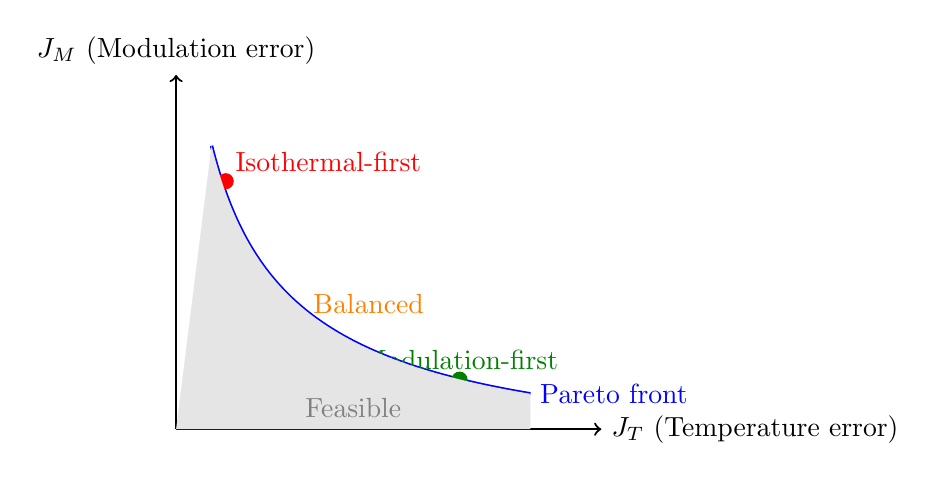
\begin{tikzpicture}[scale=0.9]
    % Axes
    \draw[thick,->] (0,0) -- (6,0) node[right] {$J_T$ (Temperature error)};
    \draw[thick,->] (0,0) -- (0,5) node[above] {$J_M$ (Modulation error)};
    
    % Pareto front
    \draw[very thick, blue] (0.5,4) .. controls (1,2) and (2,1) .. (5,0.5);
    \node[blue, right] at (5,0.5) {Pareto front};
    
    % Operating points
    \filldraw[red] (0.7,3.5) circle (3pt);
    \node[red, above right] at (0.7,3.5) {Isothermal-first};
    
    \filldraw[green!50!black] (4,0.7) circle (3pt);
    \node[green!50!black, above] at (4,0.7) {Modulation-first};
    
    \filldraw[orange] (1.8,1.5) circle (3pt);
    \node[orange, above right] at (1.8,1.5) {Balanced};
    
    % Infeasible region
    \fill[gray!20] (0,0) -- (0.5,4) .. controls (1,2) and (2,1) .. (5,0.5) -- (5,0) -- cycle;
    \node[gray] at (2.5,0.3) {Feasible};
    
\end{tikzpicture}
\caption{Pareto front showing trade-off between temperature control and modulation}
\label{fig:pareto}
\end{figure}

\subsubsection{Epsilon-Constraint Method}

An alternative formulation constrains one objective:

\begin{align}
\min_{\mathbf{u}} \quad & J_M(\mathbf{u}) \\
\text{s.t.} \quad & J_T(\mathbf{u}) \leq \epsilon_T
\end{align}

This ensures isothermal compliance ($J_T \leq \epsilon_T$) while maximizing modulation.

\subsection{Algorithm 3: Adaptive Gain Scheduling}

\subsubsection{Motivation}

System dynamics vary with operating conditions:
\begin{itemize}
\item Sample volume affects thermal mass
\item Temperature affects dielectric properties
\item Protein concentration affects folding signal
\item Solvent (H$_2$O vs.\ D$_2$O) affects heating rate
\end{itemize}

Fixed gains cannot optimally handle this variation.

\subsubsection{Scheduling Variables}

Gains are scheduled based on:

\begin{table}[h]
\centering
\begin{tabular}{lll}
\toprule
\textbf{Variable} & \textbf{Symbol} & \textbf{Effect on Gains} \\
\midrule
Temperature & $T$ & Higher $T$ $\to$ higher cooling gain \\
Power level & $P$ & Higher $P$ $\to$ higher temperature feedback gain \\
Solvent & H$_2$O/D$_2$O & D$_2$O $\to$ modified thermal gains \\
Sample volume & $V$ & Larger $V$ $\to$ slower gains (thermal inertia) \\
\bottomrule
\end{tabular}
\caption{Gain scheduling variables}
\end{table}

\subsubsection{Interpolation}

Gains are interpolated between pre-computed values:

\begin{equation}
\mathbf{K}(\sigma) = \sum_{i=1}^{N} \alpha_i(\sigma) \mathbf{K}_i
\label{eq:interp}
\end{equation}

where $\sigma$ is the scheduling variable vector and $\alpha_i$ are interpolation weights (e.g., from lookup table or polynomial).

\subsection{Algorithm 4: Model Predictive Control (MPC)}

\subsubsection{MPC Formulation}

MPC solves an optimization problem at each time step:

\begin{align}
\min_{\mathbf{u}_{0:N-1}} \quad & \sum_{k=0}^{N-1} \left[ \|\mathbf{x}_k - \mathbf{x}_{\text{ref}}\|_{\mathbf{Q}}^2 + \|\mathbf{u}_k\|_{\mathbf{R}}^2 \right] + \|\mathbf{x}_N - \mathbf{x}_{\text{ref}}\|_{\mathbf{P}}^2 \\
\text{s.t.} \quad & \mathbf{x}_{k+1} = \mathbf{A}_d\mathbf{x}_k + \mathbf{B}_d\mathbf{u}_k \\
& \mathbf{x}_k \in \mathcal{X}, \quad \mathbf{u}_k \in \mathcal{U}
\end{align}

where $N$ is the prediction horizon and $\mathcal{X}$, $\mathcal{U}$ are constraint sets.

\begin{figure}[h]
\centering
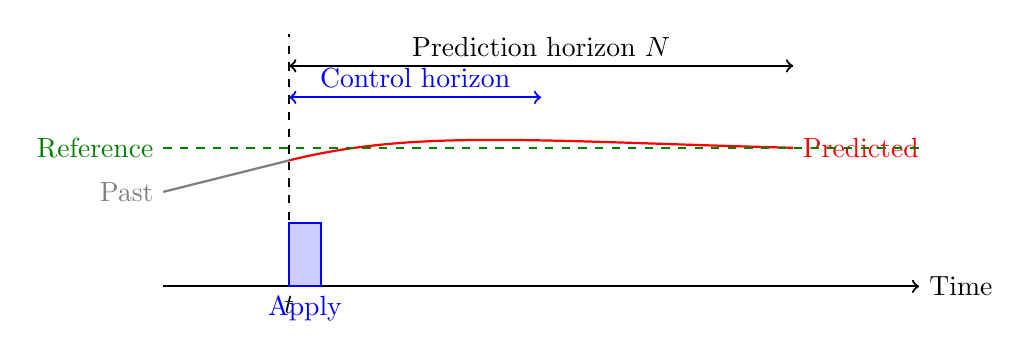
\begin{tikzpicture}[scale=0.8]
    % Time axis
    \draw[thick,->] (0,0) -- (12,0) node[right] {Time};
    
    % Current time
    \draw[thick, dashed] (2,0) -- (2,4);
    \node[below] at (2,0) {$t$};
    
    % Prediction horizon
    \draw[<->, thick] (2,3.5) -- (10,3.5);
    \node[above] at (6,3.5) {Prediction horizon $N$};
    
    % Control horizon
    \draw[<->, thick, blue] (2,3) -- (6,3);
    \node[above, blue] at (4,3) {Control horizon};
    
    % Past trajectory
    \draw[thick, gray] (0,1.5) -- (2,2);
    \node[gray, left] at (0,1.5) {Past};
    
    % Predicted trajectory
    \draw[thick, red] (2,2) .. controls (4,2.5) and (6,2.3) .. (10,2.2);
    \node[red, right] at (10,2.2) {Predicted};
    
    % Reference
    \draw[thick, green!50!black, dashed] (0,2.2) -- (12,2.2);
    \node[green!50!black, left] at (0,2.2) {Reference};
    
    % Applied control
    \draw[thick, blue, fill=blue!20] (2,0) rectangle (2.5,1);
    \node[blue, below] at (2.25,0) {Apply};
    
\end{tikzpicture}
\caption{Model Predictive Control: prediction horizon and receding horizon implementation}
\label{fig:mpc}
\end{figure}

\subsubsection{Thermal-Optical Model}

The MPC uses a simplified thermal-optical model:

\begin{align}
C_s \frac{dT}{dt} &= \alpha P_{\text{MW}} - k_{\text{cool}}(T - T_{\text{amb}}) - P_{\text{cool}} \label{eq:thermal} \\
\frac{dM}{dt} &= \beta(f - f_{\text{res}})^{-2} \cdot P_{\text{MW}} - \gamma M \label{eq:modulation}
\end{align}

where:
\begin{itemize}
\item $C_s$ = sample heat capacity
\item $\alpha$ = microwave absorption coefficient
\item $k_{\text{cool}}$ = passive cooling rate
\item $\beta$ = resonant coupling strength
\item $f_{\text{res}}$ = resonance frequency
\item $\gamma$ = modulation decay rate
\end{itemize}

\subsubsection{Real-Time Implementation}

For real-time operation, the MPC optimization is solved using:
\begin{enumerate}[label=(\arabic*)]
\item Quadratic programming (QP) solvers (e.g., OSQP, qpOASES)
\item Explicit MPC (pre-computed piecewise affine control law)
\item Neural network approximation of optimal policy
\end{enumerate}

Typical solution time: $<$ 1 ms for prediction horizon $N = 20$.

\subsection{Algorithm 5: Constraint Satisfaction}

\subsubsection{Constraint Types}

\begin{table}[h]
\centering
\begin{tabular}{lll}
\toprule
\textbf{Constraint} & \textbf{Expression} & \textbf{Limit} \\
\midrule
Temperature deviation & $|T - T_{\text{set}}|$ & $< 0.5^\circ$C (hard), $< 0.1^\circ$C (soft) \\
Microwave power & $P_{\text{MW}}$ & $0 \leq P \leq P_{\text{max}}$ \\
Cooling power & $P_{\text{cool}}$ & $0 \leq P \leq P_{\text{cool,max}}$ \\
Frequency range & $f$ & $f_{\text{min}} \leq f \leq f_{\text{max}}$ \\
Power rate of change & $|\dot{P}|$ & $< \dot{P}_{\text{max}}$ \\
Temperature rate & $|\dot{T}|$ & $< 1^\circ$C/s \\
\bottomrule
\end{tabular}
\caption{System constraints}
\end{table}

\subsubsection{Hard vs.\ Soft Constraints}

\begin{enumerate}[label=(\alph*)]
\item \textbf{Hard constraints:} Must never be violated. Implemented as inequality constraints in optimization.

\item \textbf{Soft constraints:} Violation incurs penalty but is allowed. Implemented as slack variables:
\begin{equation}
|T - T_{\text{set}}| \leq \epsilon_T + s_T, \quad s_T \geq 0
\end{equation}
with penalty $w_s s_T^2$ added to cost function.
\end{enumerate}

\subsubsection{Safety Interlocks}

Independent of the optimization, hardware interlocks enforce:
\begin{enumerate}[label=(\arabic*)]
\item Emergency shutdown if $T > T_{\text{max}}$
\item Power cutoff if cooling fails
\item Frequency limits enforced in hardware
\end{enumerate}

\begin{figure}[h]
\centering
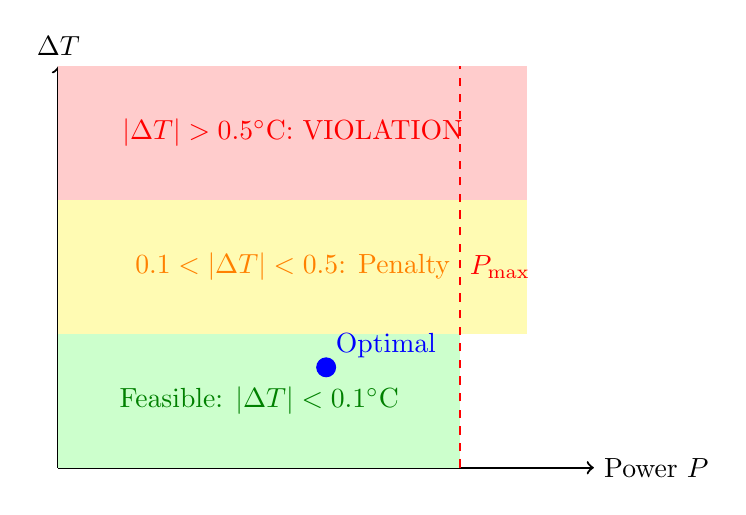
\begin{tikzpicture}[scale=0.85]
    % Axes
    \draw[thick,->] (0,0) -- (8,0) node[right] {Power $P$};
    \draw[thick,->] (0,0) -- (0,6) node[above] {$\Delta T$};
    
    % Hard constraint region
    \fill[red!20] (0,4) rectangle (7,6);
    \node[red] at (3.5,5) {$|\Delta T| > 0.5^\circ$C: VIOLATION};
    
    % Soft constraint region
    \fill[yellow!30] (0,2) rectangle (7,4);
    \node[orange] at (3.5,3) {$0.1 < |\Delta T| < 0.5$: Penalty};
    
    % Feasible region
    \fill[green!20] (0,0) rectangle (6,2);
    \node[green!50!black] at (3,1) {Feasible: $|\Delta T| < 0.1^\circ$C};
    
    % Power limit
    \draw[thick, red, dashed] (6,0) -- (6,6);
    \node[red, right] at (6,3) {$P_{\text{max}}$};
    
    % Operating point
    \filldraw[blue] (4,1.5) circle (4pt);
    \node[blue, above right] at (4,1.5) {Optimal};
    
\end{tikzpicture}
\caption{Constraint satisfaction regions in power--temperature space}
\label{fig:constraints}
\end{figure}

\subsection{Algorithm 6: Resonance Tracking}

\subsubsection{Motivation}

The resonance frequency may drift due to:
\begin{itemize}
\item Temperature changes affecting dielectric properties
\item Sample composition changes during folding
\item Equipment drift
\end{itemize}

\subsubsection{Extremum Seeking Control}

A sinusoidal perturbation is added to the frequency:

\begin{equation}
f(t) = f_0 + a \sin(\omega_p t)
\label{eq:extremum}
\end{equation}

The folding signal is demodulated at $\omega_p$ to estimate the gradient:

\begin{equation}
\frac{\partial M}{\partial f} \approx \frac{2}{a} \langle M(t) \sin(\omega_p t) \rangle
\label{eq:gradient}
\end{equation}

The center frequency is updated:

\begin{equation}
\dot{f}_0 = \gamma_f \frac{\partial M}{\partial f}
\label{eq:freq_update}
\end{equation}

\subsubsection{Resonance Tracking Loop}

\begin{enumerate}[label=(\arabic*)]
\item Apply frequency perturbation (amplitude $a \sim 0.01$ GHz, frequency $\omega_p \sim 10$ Hz)
\item Measure folding signal $M(t)$
\item Demodulate to extract gradient
\item Update center frequency to move toward resonance peak
\item Repeat continuously during operation
\end{enumerate}

\subsection{Algorithm 7: Isotope-Mode Automatic Reconfiguration}

\subsubsection{Mode Detection}

The controller automatically detects solvent:

\begin{enumerate}[label=(\alph*)]
\item \textbf{Manual selection:} Operator specifies H$_2$O or D$_2$O
\item \textbf{Dielectric sensing:} Measure dielectric constant at reference frequency
\item \textbf{Resonance scan:} Identify resonance frequency (14.65 vs.\ 10.4 GHz)
\end{enumerate}

\subsubsection{Reconfiguration Actions}

When switching from H$_2$O to D$_2$O mode:

\begin{table}[h]
\centering
\begin{tabular}{lll}
\toprule
\textbf{Parameter} & \textbf{H$_2$O Mode} & \textbf{D$_2$O Mode} \\
\midrule
Operating frequency & 14.65 GHz & 10.4 GHz \\
Frequency sweep range & 12--17 GHz & 8--13 GHz \\
Thermal model $\alpha$ & $\alpha_{\text{H}_2\text{O}}$ & $\alpha_{\text{D}_2\text{O}} \approx 0.9\alpha_{\text{H}_2\text{O}}$ \\
Cooling gain & $K_{\text{cool}}$ & $K_{\text{cool}} \times 1.1$ \\
\bottomrule
\end{tabular}
\caption{Parameter reconfiguration for isotope mode}
\end{table}

\subsection{Implementation Considerations}

\subsubsection{Computation Platforms}

\begin{table}[h]
\centering
\begin{tabular}{lll}
\toprule
\textbf{Platform} & \textbf{Advantages} & \textbf{Disadvantages} \\
\midrule
Embedded MCU & Low cost, low power & Limited computation \\
FPGA & Fast, deterministic & Complex development \\
Host PC & Flexible, powerful & Latency, reliability \\
DSP & Real-time optimized & Moderate cost \\
\bottomrule
\end{tabular}
\caption{Implementation platforms}
\end{table}

\subsubsection{Recommended Architecture}

\begin{enumerate}[label=(\arabic*)]
\item \textbf{Inner loop (1 kHz):} PID temperature control on embedded MCU
\item \textbf{Outer loop (100 Hz):} MIMO/MPC on DSP or host PC
\item \textbf{Supervisory (10 Hz):} Mode selection, gain scheduling on host PC
\end{enumerate}

\subsubsection{Communication}

\begin{itemize}
\item Inner loop to outer loop: Low-latency link (SPI, LVDS)
\item Outer loop to supervisory: Ethernet or USB
\item All loops: Shared memory or message passing
\end{itemize}

\subsection{Performance Specifications}

\begin{table}[h]
\centering
\begin{tabular}{lll}
\toprule
\textbf{Metric} & \textbf{Specification} & \textbf{Notes} \\
\midrule
Temperature tracking & $|\Delta T| < 0.1^\circ$C RMS & Isothermal compliance \\
Modulation achieved & $M > 30\%$ & At resonance \\
Control bandwidth & $>$ 100 Hz & For pulsed operation \\
Frequency tracking & $\pm$0.05 GHz & Resonance lock \\
Mode switch time & $<$ 1 s & H$_2$O $\leftrightarrow$ D$_2$O \\
Computation latency & $<$ 1 ms & Real-time constraint \\
\bottomrule
\end{tabular}
\caption{Control system performance specifications}
\end{table}

\newpage

%% ============================================================================
%%                              CLAIMS
%% ============================================================================

\section{CLAIMS}

What is claimed is:

\subsection{MIMO Feedback Control Claims}

\begin{enumerate}[label=\textbf{\arabic*.}]

\item A method for closed-loop control of a protein folding modulation apparatus, comprising:
\begin{enumerate}[label=(\alph*)]
\item measuring a temperature of a sample using a temperature sensor;
\item measuring a folding signal of the sample using a folding detector;
\item computing control outputs based on temperature error and folding error using a multi-input multi-output (MIMO) controller;
\item adjusting microwave power, cooling power, and frequency based on the control outputs; and
\item repeating steps (a) through (d) in a closed loop.
\end{enumerate}

\item The method of claim 1, wherein the MIMO controller uses a state-space feedback formulation with a gain matrix $\mathbf{K}$ designed using Linear Quadratic Regulator (LQR) theory.

\item The method of claim 1, wherein the control loop operates at a rate of at least 100 Hz.

\item The method of claim 1, wherein the method maintains temperature deviation $|\Delta T| < 0.1^\circ$C while achieving folding modulation $M > 30\%$.

\end{enumerate}

\subsection{Multi-Objective Optimization Claims}

\begin{enumerate}[label=\textbf{\arabic*.}]
\setcounter{enumi}{4}

\item A method for multi-objective control of protein folding modulation, comprising:
\begin{enumerate}[label=(\alph*)]
\item defining a first objective to minimize temperature deviation from a setpoint;
\item defining a second objective to maximize folding modulation;
\item computing control outputs that optimize a weighted combination of the first and second objectives; and
\item adjusting weights to select an operating point on a Pareto front.
\end{enumerate}

\item The method of claim 5, wherein the weighted combination is $J = \lambda J_T + (1-\lambda) J_M$ with $\lambda \in [0, 1]$.

\item The method of claim 5, further comprising an operating mode selection from:
\begin{enumerate}[label=(\roman*)]
\item isothermal-first mode with temperature deviation prioritized;
\item modulation-first mode with folding modulation prioritized; and
\item balanced mode with equal priority.
\end{enumerate}

\item The method of claim 5, wherein the optimization is solved using epsilon-constraint method with isothermal compliance as a hard constraint.

\end{enumerate}

\subsection{Adaptive Control Claims}

\begin{enumerate}[label=\textbf{\arabic*.}]
\setcounter{enumi}{8}

\item A method for adaptive control of protein folding modulation, comprising:
\begin{enumerate}[label=(\alph*)]
\item measuring operating conditions including temperature, power level, and sample properties;
\item selecting control gains from a pre-computed set based on the operating conditions;
\item interpolating between gains for smooth transitions; and
\item applying the adapted gains to the control algorithm.
\end{enumerate}

\item The method of claim 9, wherein the operating conditions include solvent type (H$_2$O or D$_2$O).

\item The method of claim 9, wherein gains are interpolated using polynomial or lookup table methods.

\end{enumerate}

\subsection{Model Predictive Control Claims}

\begin{enumerate}[label=\textbf{\arabic*.}]
\setcounter{enumi}{11}

\item A method for model predictive control of protein folding modulation, comprising:
\begin{enumerate}[label=(\alph*)]
\item using a thermal-optical model to predict sample temperature and folding signal over a prediction horizon;
\item solving an optimization problem to find control inputs that minimize a cost function over the prediction horizon;
\item applying the first control input from the optimal sequence;
\item advancing the prediction horizon by one step; and
\item repeating steps (a) through (d) in a receding horizon manner.
\end{enumerate}

\item The method of claim 12, wherein the thermal-optical model comprises:
\begin{enumerate}[label=(\roman*)]
\item a thermal model relating microwave power and cooling power to sample temperature; and
\item an optical model relating irradiation frequency and power to folding modulation.
\end{enumerate}

\item The method of claim 12, wherein the optimization problem is solved using quadratic programming with a solution time of less than 1 millisecond.

\item The method of claim 12, wherein the prediction horizon is 10 to 50 time steps.

\end{enumerate}

\subsection{Constraint Satisfaction Claims}

\begin{enumerate}[label=\textbf{\arabic*.}]
\setcounter{enumi}{15}

\item A method for constraint-aware control of protein folding modulation, comprising:
\begin{enumerate}[label=(\alph*)]
\item defining hard constraints including maximum temperature deviation and power limits;
\item defining soft constraints with associated penalty functions;
\item solving a constrained optimization problem that satisfies hard constraints and minimizes soft constraint violations; and
\item implementing hardware safety interlocks independent of the optimization.
\end{enumerate}

\item The method of claim 16, wherein the hard constraint on temperature deviation is $|\Delta T| < 0.5^\circ$C.

\item The method of claim 16, wherein soft constraints include a target temperature deviation of $|\Delta T| < 0.1^\circ$C with a quadratic penalty for violation.

\end{enumerate}

\subsection{Resonance Tracking Claims}

\begin{enumerate}[label=\textbf{\arabic*.}]
\setcounter{enumi}{18}

\item A method for automatic resonance tracking during protein folding modulation, comprising:
\begin{enumerate}[label=(\alph*)]
\item adding a sinusoidal frequency perturbation to the operating frequency;
\item measuring the folding signal response;
\item demodulating the response at the perturbation frequency to estimate the frequency gradient;
\item adjusting the center frequency in the direction of increasing folding signal; and
\item repeating steps (a) through (d) to maintain lock on the resonance peak.
\end{enumerate}

\item The method of claim 19, wherein the perturbation amplitude is 0.01 to 0.1 GHz and the perturbation frequency is 1 to 100 Hz.

\item The method of claim 19, wherein the frequency is maintained within $\pm$0.05 GHz of the resonance peak.

\end{enumerate}

\subsection{Isotope Mode Claims}

\begin{enumerate}[label=\textbf{\arabic*.}]
\setcounter{enumi}{21}

\item A method for automatic reconfiguration of control parameters for isotope mode operation, comprising:
\begin{enumerate}[label=(\alph*)]
\item detecting the solvent type as H$_2$O or D$_2$O;
\item reconfiguring the operating frequency to approximately 14.65 GHz for H$_2$O or 10.4 GHz for D$_2$O;
\item adjusting thermal model parameters for the detected solvent;
\item adjusting control gains for the detected solvent; and
\item continuing closed-loop control with the reconfigured parameters.
\end{enumerate}

\item The method of claim 22, wherein solvent detection is performed by one or more of:
\begin{enumerate}[label=(\roman*)]
\item manual operator input;
\item dielectric constant measurement; and
\item resonance frequency identification.
\end{enumerate}

\end{enumerate}

\subsection{System Claims}

\begin{enumerate}[label=\textbf{\arabic*.}]
\setcounter{enumi}{23}

\item A control system for protein folding modulation, comprising:
\begin{enumerate}[label=(\alph*)]
\item a temperature sensor configured to measure sample temperature;
\item a folding detector configured to measure folding signal;
\item a processor configured to execute a closed-loop control algorithm according to any of claims 1--23;
\item a microwave power controller responsive to the processor;
\item a cooling system controller responsive to the processor; and
\item a frequency controller responsive to the processor.
\end{enumerate}

\item The system of claim 24, comprising a hierarchical architecture with:
\begin{enumerate}[label=(\roman*)]
\item an inner loop operating at 1 kHz for temperature control;
\item an outer loop operating at 100 Hz for MIMO/MPC control; and
\item a supervisory loop operating at 10 Hz for mode selection and adaptation.
\end{enumerate}

\item A non-transitory computer-readable medium storing instructions that, when executed by a processor, cause the processor to perform the method of any of claims 1--23.

\end{enumerate}

\newpage

%% ============================================================================
%%                         ABSTRACT
%% ============================================================================

\section*{ABSTRACT}
\addcontentsline{toc}{section}{ABSTRACT}

Control algorithms for closed-loop operation of protein folding modulation apparatus enabling simultaneous isothermal maintenance and resonant modulation maximization. The algorithms comprise: (1) multi-input multi-output (MIMO) feedback control using temperature and folding signal readouts to adjust microwave power, frequency, and cooling power with gains designed using Linear Quadratic Regulator (LQR) theory; (2) multi-objective optimization minimizing temperature deviation while maximizing folding modulation, with configurable weighting and Pareto-optimal operating point selection; (3) adaptive gain scheduling adjusting control parameters based on temperature, power level, sample volume, and solvent type; (4) model predictive control (MPC) using a thermal-optical model to predict system response over a receding horizon; (5) constraint satisfaction ensuring temperature bounds ($|\Delta T| < 0.1^\circ$C target, $< 0.5^\circ$C hard limit), power limits, and safety interlocks; (6) resonance tracking using extremum seeking control with sinusoidal frequency perturbation to maintain lock on the resonance peak; and (7) isotope-mode automatic reconfiguration for H$_2$O (14.65 GHz) and D$_2$O (10.4 GHz) operation. Implementation uses hierarchical architecture with inner loop (1 kHz) for temperature, outer loop (100 Hz) for MIMO/MPC, and supervisory loop (10 Hz) for adaptation. Applications include automated protein folding modulation for research, manufacturing quality control, and therapeutic intervention.

\vspace{1in}

\begin{center}
\textbf{--- END OF SPECIFICATION ---}
\end{center}

\newpage

%% ============================================================================
%%                         INVENTOR DECLARATION
%% ============================================================================

\section*{INVENTOR DECLARATION}
\addcontentsline{toc}{section}{INVENTOR DECLARATION}

I, Jonathan Washburn, declare that:

\begin{enumerate}[label=(\arabic*)]
\item I am the original and sole inventor of the control algorithms described and claimed in this application.

\item I have reviewed the above specification and claims and believe them to be accurate and complete.

\item I believe the claimed invention to be novel, useful, and non-obvious over the prior art.

\item I authorize the filing of this provisional patent application to establish a priority date.
\end{enumerate}

\vspace{1in}

\noindent\textbf{Inventor Signature:} \hrulefill

\vspace{0.5in}

\noindent\textbf{Name:} Jonathan Washburn

\noindent\textbf{Email:} washburn.jonathan@gmail.com

\noindent\textbf{Date:} \hrulefill

\vspace{1in}

\begin{center}
\textit{This document is intended for provisional patent application filing purposes.\\
All information contained herein is confidential and proprietary.}
\end{center}

\end{document}
